\documentclass{article}
\usepackage{style}
\title{CHE374 Cheatsheet}
\author{Hanhee Lee}
\lhead{CHE374}
\rhead{Hanhee Lee}

\begin{document}
    \maketitle
    \tableofcontents
    \section{Chapter 1}
    \section{Chapter 2}
    \section{Chapter 3}

% Process
\begin{process}
    Hanhee Lee
\end{process}

% Example 
\begin{example}
    Hanhee Lee
\end{example}

% Definition
\begin{definition}
    Hanhee Lee 
\end{definition}

% Theorem
\begin{theorem}
    Hanhee Lee
\end{theorem}

% Derivation
\begin{derivation}
    Hanhee Lee
\end{derivation}

% Intuition
\begin{intuition}
    Hanhee Lee
\end{intuition}

% Warning
\begin{warning}
    Hanhee Lee
\end{warning}

% Insert Image 
\begin{figure}[H]
    \centering
    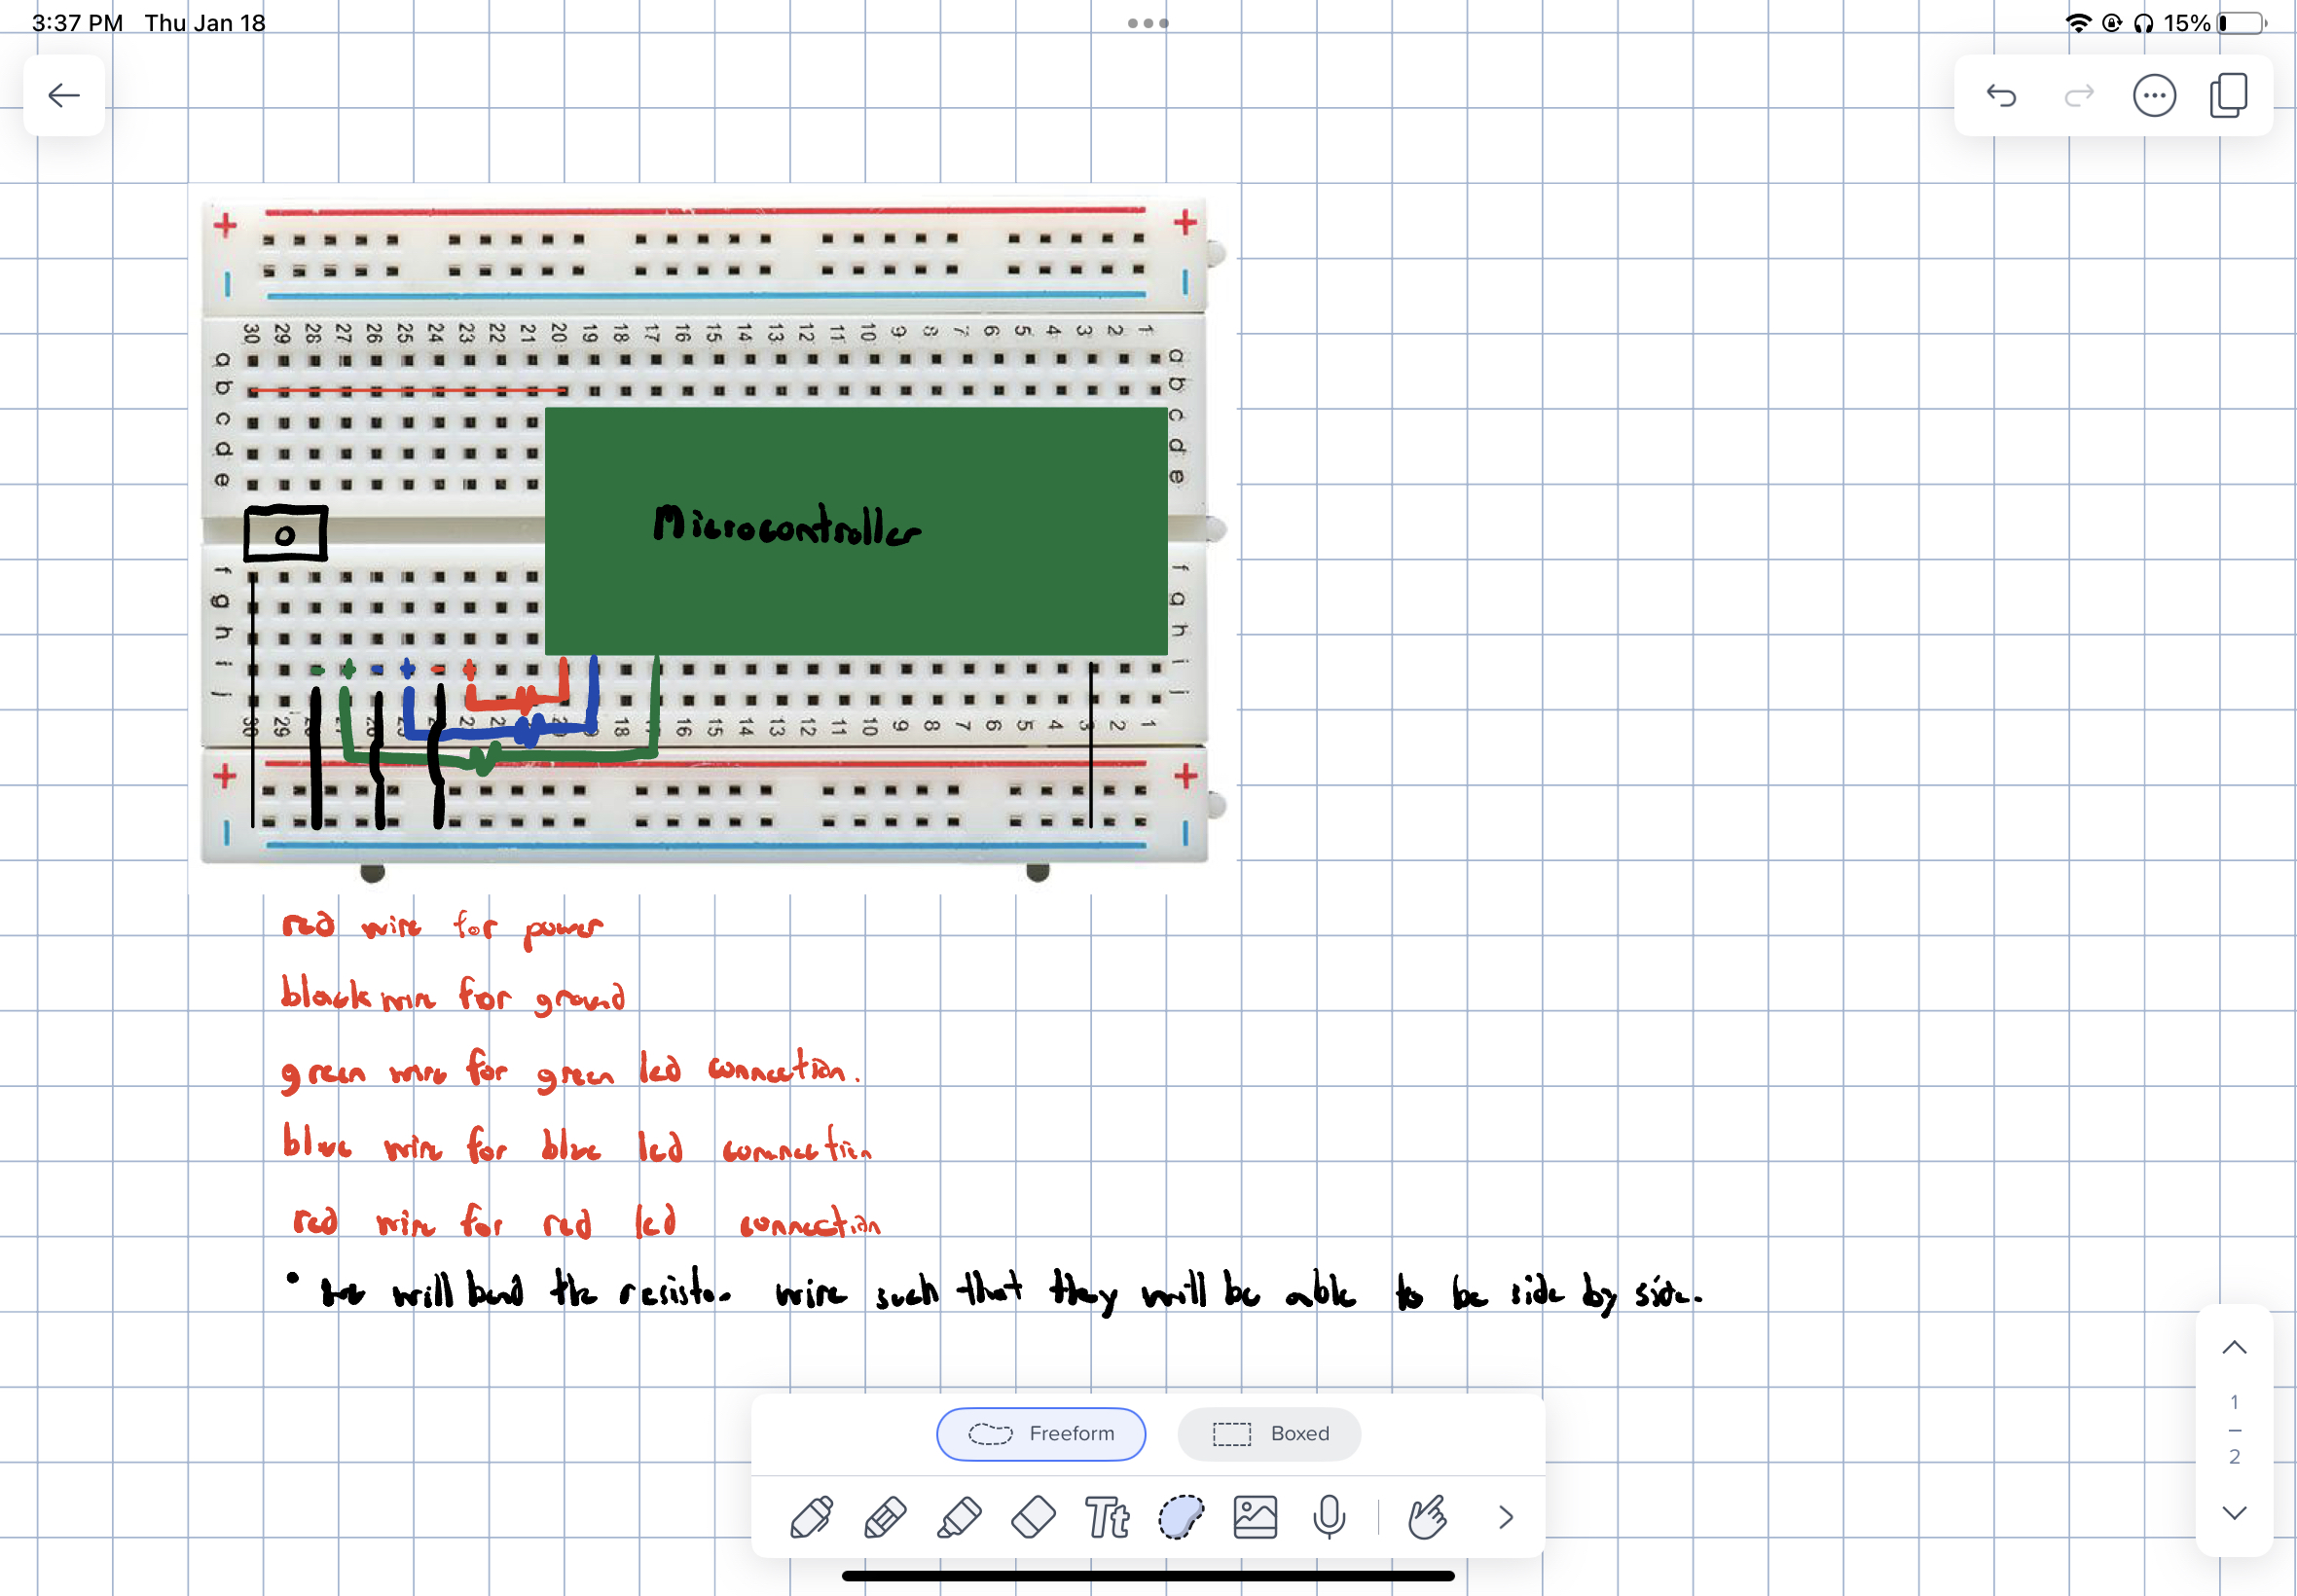
\includegraphics[width=0.5\textwidth]{00_Images/diagram_circuit.png}
    \caption{ESC195}
\end{figure}

\end{document}